\documentclass[12pt]{extarticle}
\usepackage{graphicx}
\usepackage[utf8]{inputenc}
\usepackage{cite}

\title{Proposal}
\author{
Hanzhou Tang \\
\texttt{hanzhout@smu.edu}
\and 
Jiutian Yu \\
\texttt{jiutiany@smu.com}
}
\date{February 2019}
\begin{document}
\maketitle
    \begin{abstract}
        We want to build an assembly simulator which should support basic x86 assembly instructions.
        \end{abstract}
        \section{Motivation}
        To implement a basic architecture is a direct way to reflect what we are going to learn in this class. We could also say we are going to implement a simple virtual machine. Beyond simply implementing the original proposal, we want to add some new functions based on this class to complete the architecture.  
        \section{Why Java}
        It's tempted to implement an assembly simulator in a low level language like C or C++. However, after some considerations, we decided to choose Java.
        There are several reasons which will be show below. 
        \subsection{Java is easy for memory management}
        With C++11, it has smarter pointers to make life easier \cite{josuttis2012c++}. 
        However, it's implemented in library level instead of language supporting.
        Sometimes, when we mistakenly mixed raw pointers and smart pointers , smart pointers may become useless.
        \subsection{Java is easy to test}
        There are lots of powerful java testing framework to do unit test. For example, JUnit or Groovy Spock. 
        Meanwhile, because Java support proxy object, it's much easy to mock objects and record function invoking.
        \subsection{Java is easy for package manage}
        With the help of gradle \cite{muschko2014gradle}, it's very easy for us to import different libraries and do deployment. We believe it could save us lots of time and efforts.
        \subsection{Java is easy to integrate with REST API}
        If we could finish our project well, we may want to implement an online version for all users. We could easily provide REST API with the help of Spring \cite{walls2005spring}.
        \section{Our registers}
        We do want to implement some basic functionality of x86 platform. So we decide to imitate ten 32 bits registers. A table, which is Table1, of our registers is shown below.
        The table originally comes from \cite{kusswurm2014modern}.
        As you can see, we ignore all segment registers. The reason is that according to our design, only one process can run at one time and no context switch.
        We think, in this case, segment information is unnecessary. Maybe we're wrong, we may change our decision later.  
        \section{Our instruction set}
        We want to support a subset of assembly instructions on x86 platform. 
        By doing some researches \cite{kusswurm2014modern}, we provide a table which contains all instructions we want to support.
        \section{Design}
        For now, we decided to split the project into 3 components. They are assembler, instructions and virtual machine. 
        \subsection{assembler}
        We based on Microsoft XASM assembler and followed its' convention and directives. However, because our time and ability is limited, we cannot implement all features in XASM. 
        But we at least want to implement the basic functionality, for example, the ability of define different segments, the ability of some basic directives, like \$ and proc. 
        We divided our assembler into 2 parts. One part is a lexer, which is responsible for tokenizing input asm file. Another part is a parser, which is responsible for convert tokens into machine codes. 
        After we finishing our assembler, it shall be able to read asm file and convert it into a binary file which contains data and machine code. (The format of machine code is defined by ourselves for convenience).
        From now on, we do finish the lexer part and currently working on parser part. If we have enough luck, we can finish parser in the spring off. 
        
        Here is a screenshot of outputs from our lexer.
        \begin{figure}[h]
            \centering
            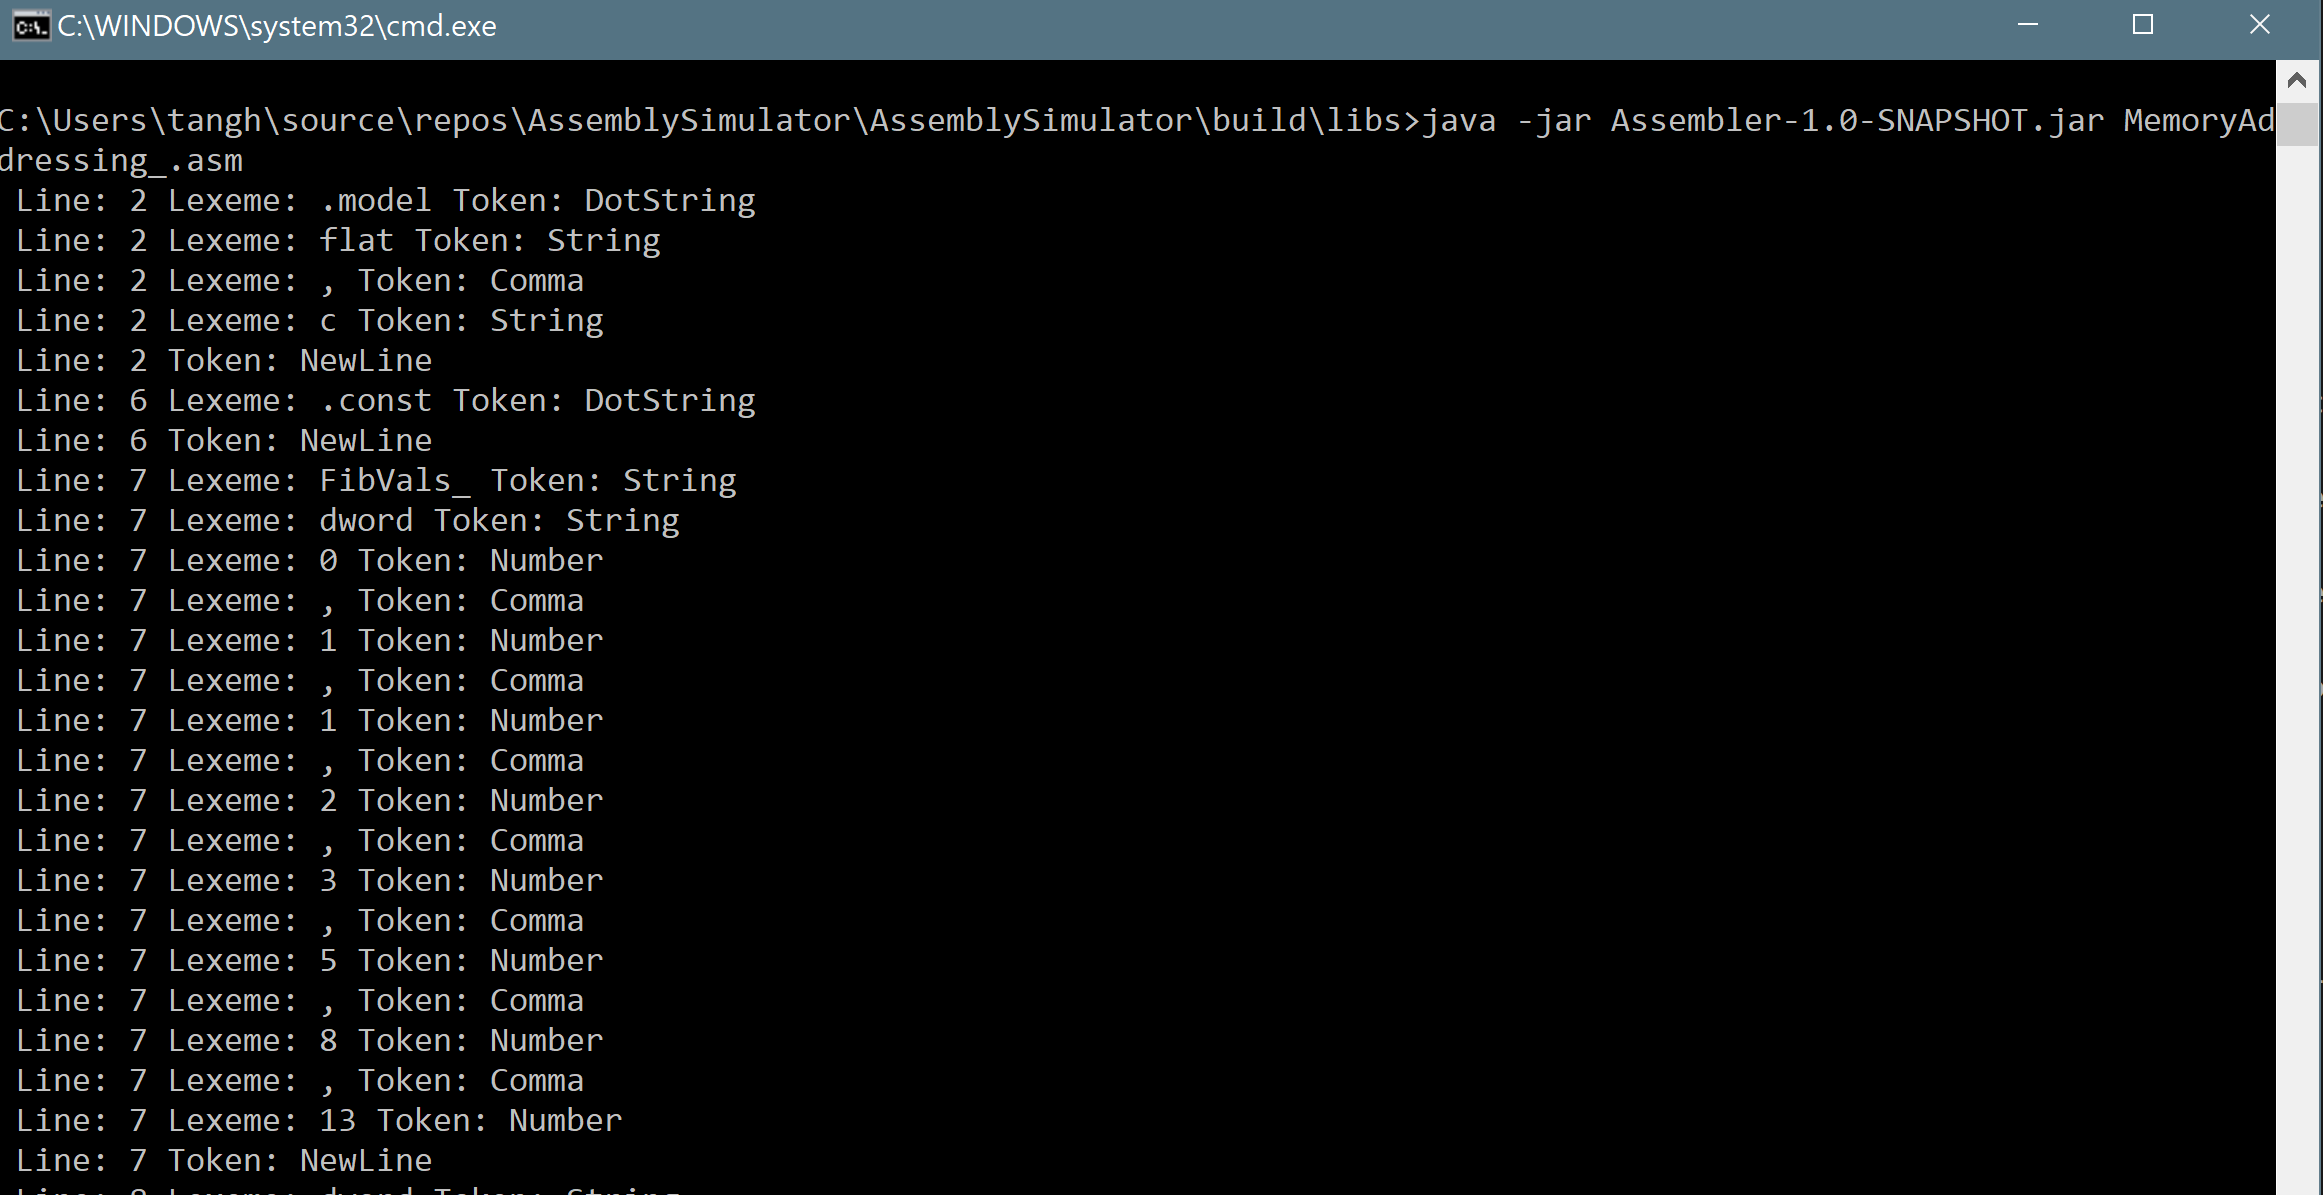
\includegraphics[width=0.7\textwidth]{screenShot.png}
            \caption{Outputs from our lexer}
        \end{figure}
        The whole asm file and output are attached in our report.
        \subsection{Instructions}
        As we said before, we want to convert asm file into binary file, which means we need design format of machine codes. We followed the convention, all machine codes are converted into 4 byte machine codes.
        For assembler, we write the instructions into binary file. For virtual machine, we load instructions from binary file. This should be the common part of assembler and virtual machine. 
        \subsection{Virtual Machine}
        The basic functionality of our virtual machine is loading the binary file and executing it. 
        We don't care about performance and optimization for our virtual machine, which means the effectiveness of our virtual machine may be pretty low. 
        However, we want to implement 5 stage pipeline in our virtual machine to show what we are learning from the Architecture class.
        Later, we may add more staffs into our virtual machine if we have time, like branch prediction. 
        We think the virtual machine is really not easy to implement, thus we plan to focus more in this part. 

        \section{To do}
        \begin{enumerate}
        \item We need to transfer assembly files to binary files.
        \item We need our simulator is able to read these files.
        \item If we have time, we can add one LRU cache to our simulator to optimize the storages. We can also implement something having a strong connection with what we learn in this class
        \end{enumerate}

        % \section{Attachment}
        % \begin{enumerate}
        %     \item A visual studio solution which contains some asm files. Those asm file will be our testing target. These files came from \cite{kusswurm2014modern} and we made tiny modifications.
        %     \item A Java project of our assembler, this part is not done yet. We are currently working on it. However, the lexer is finished.
        %     \item A built jar file of our assembler. 
        %     \item The report.
        % \end{enumerate}




        \begin{table}[h!]
            \centering
            \begin{tabular}{||c | p{9cm}||} 
             \hline
             Register & Descriptions \\ [0.5ex] 
             \hline
             EAX & Accumulator. 0 to 7 can be refered as AL. 8 to 15 can be refered as AH. 0 to 15 can be refered as AX. \\ 
             \hline
             EBX & Memory pointer, base Register. 0 to 7 can be refered as BL. 8 to 15 can be refered as BH. 0 to 15 can be refered as BX. \\
             \hline
             ECX & Loop control. 0 to 7 can be refered as CL. 8 to 15 can be refered as CH. 0 to 15 can be refered as CX. \\
             \hline
             EDX & Integer multiplication, integer division. 0 to 7 can be refered as DL. 8 to 15 can be refered as DH. 0 to 15 can be refered as DX. \\
             \hline
             ESI & String instruction source pointer. \\
             \hline
             EDI & String instruction destination pointer. \\
             \hline
             ESP & Stack Pointer. \\
             \hline
             EBP & Stack frame base Pointer. \\
             \hline
             EIP & Instruction pointer register. \\
             \hline
             EFLAGS & Flag register. \\
             \hline
            \end{tabular}
            \caption{The registers we want to imitate}
            \label{table:1}
        \end{table}
        
        \begin{table}[h!]
            \centering
            \begin{tabular}{||c | p{9cm}||} 
             \hline
             mov & Copy data from one place to another place. \\ [0.5ex] 
             \hline
             push & Push register, memory location or immediate value onto stack.  \\ 
             \hline
             pop & Pop the first item from stack. \\
             \hline
             add & Add two number \\
             \hline
             sub &  Subtraction \\
             \hline
             cbw & Sign-extends register AL. \\
             \hline
             cwd & Sign-extends register AX. \\
             \hline
             bswap & Reverse the bytes of a 32-bit register. \\
             \hline
             and & Logic and. \\
             \hline
             or & Logic or. \\
             \hline
             xor & Logic xor. \\
             \hline
             not & Logic not. \\
             \hline
             sal/shl & Left shift. \\
             \hline
             sar & Arithmetric right shift. \\
             \hline
             shr & Logic right shift. \\
             \hline
             cmpsb/cmpsw/cmpsd & Compare the values at location. \\
             \hline
             lodsb/lodsw/lodsd & Loads the values at location. \\
             \hline
             stosb/stosw/stosd & Save the values at register to memory. \\
             \hline
             rep/repne & Repeat a specified instruction by condition \\
             \hline
             jmp/jcc/jecxz & Unconditonal/conditional jump \\
             \hline
             call & Push content to stack then do unconditonal jump.\\
             \hline
             ret & Pop stack then do unconditonal jump.\\
             \hline
             enter & Create a stack frame for function.\\
             \hline
             leave & Remove a stack frame of function.\\
             \hline
             loop/loope/loopz/loopne/loopnz & Loop.\\
             \hline
             nop & Advance the instruction pointer.\\
             \hline
            \end{tabular}
            \caption{The instructions we want to imitate}
            \label{table:2}
        \end{table}


\bibliography{main}{}
\bibliographystyle{acm}


\end{document}
